\documentclass[leqno]{article}
\usepackage[utf8]{inputenc}
\usepackage{enumitem}
\usepackage{tikz}
\usepackage[parfill]{parskip} % Don't start new paragraph with tab.
\usepackage{amsmath} % For \tag and \eqref

\title{Computationele logica}
\author{
    Kamans, Jim\\
    \texttt{10302905}
    \and
    Roosingh, Sander\\
    \texttt{11983957}
    \and
    Schenk, Stefan\\
    \texttt{11881798}
}
\date{November 2017}

\begin{document}

\maketitle


%%%%%%%%%%%%%%%%
%% Exercise 1 %%
%%%%%%%%%%%%%%%%
\section*{Exercise 1}

\begin{enumerate}

    \item The sentence $\theta$ encoding all information: \\

    The Queen knows the following: \\
    Alice knows Bob has a red hat. Alice knows Bob doesn't know it, and she
    knows the Queen knows this. Alice doesn't know her own hat. \\
    Bob knows Alice has a red hat. Bob knows Alice doesn't know it, and he
    knows the Queen knows this. Bob doesn't know his own hat. \\

    $\theta$ =
        $K_q (
        K_a (
            r_b \wedge
            \neg K_b (r_b \vee w_b) \wedge
            K_q ((r_a \vee r_w) \wedge (r_b \vee r_w))
        )
        \wedge \neg K_a (r_a \vee w_a)
        \wedge
        K_b (
            r_a \wedge
            \neg K_a (r_a \vee w_a) \wedge
            K_q ((r_a \vee r_w) \wedge (r_b \vee r_w))
        )
        \wedge \neg K_b (r_b \vee w_b)
        )$

    \item A representation of the situation model \textbf{M}: \\

    $\mathcal{A}$ = \{a, b, q\} the agents Alice, Bob, and the Queen \\
    $\Phi$ = $\{r_a, w_a, r_b, w_b\}$ written as WR for:
    a is white and b is red \\

    \begin{center}
    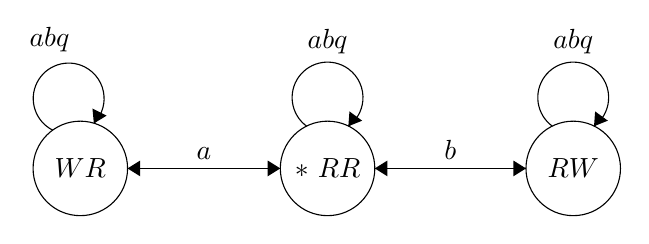
\begin{tikzpicture}[scale=0.2]
    \tikzstyle{every node}+=[inner sep=0pt]
    \draw [black] (38.4,-13.7) circle (3);
    \draw (38.4,-13.7) node {$*\mbox{ }RR$};
    \draw [black] (54,-13.7) circle (3);
    \draw (54,-13.7) node {$RW$};
    \draw [black] (22.7,-13.7) circle (3);
    \draw (22.7,-13.7) node {$WR$};
    \draw [black] (41.4,-13.7) -- (51,-13.7);
    \fill [black] (51,-13.7) -- (50.2,-13.2) -- (50.2,-14.2);
    \draw (46.2,-13.2) node [above] {$b$};
    \draw [black] (51,-13.7) -- (41.4,-13.7);
    \fill [black] (41.4,-13.7) -- (42.2,-14.2) -- (42.2,-13.2);
    \draw [black] (35.4,-13.7) -- (25.7,-13.7);
    \fill [black] (25.7,-13.7) -- (26.5,-14.2) -- (26.5,-13.2);
    \draw (30.55,-13.2) node [above] {$a$};
    \draw [black] (25.7,-13.7) -- (35.4,-13.7);
    \fill [black] (35.4,-13.7) -- (34.6,-13.2) -- (34.6,-14.2);
    \draw [black] (37.077,-11.02) arc (234:-54:2.25);
    \draw (38.4,-6.45) node [above] {$abq$};
    \fill [black] (39.72,-11.02) -- (40.6,-10.67) -- (39.79,-10.08);
    \draw [black] (52.677,-11.02) arc (234:-54:2.25);
    \draw (54,-6.45) node [above] {$abq$};
    \fill [black] (55.32,-11.02) -- (56.2,-10.67) -- (55.39,-10.08);
    \draw [black] (20.955,-11.274) arc (243.46232:-44.53768:2.25);
    \draw (20.74,-6.36) node [above] {$abq$};
    \fill [black] (23.56,-10.84) -- (24.37,-10.35) -- (23.47,-9.9);
    \end{tikzpicture}
    \end{center}

    This is an epistemic model: YES \\

    \pagebreak

    \item Seperately a and b look in their mirrors and see their red hats, the
    queen sees everything, represented in the event model $\Sigma$ with four
    actions: \\

    \begin{center}
    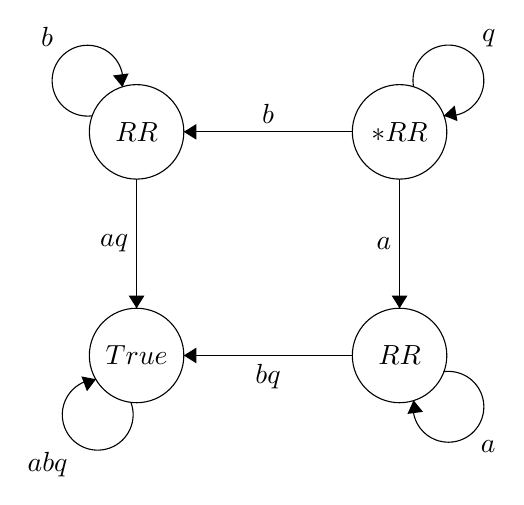
\begin{tikzpicture}[scale=0.2]
    \tikzstyle{every node}+=[inner sep=0pt]
    \draw [black] (54,-42.2) circle (3);
    \draw (54,-42.2) node {$RR$};
    \draw [black] (37.3,-28) circle (3);
    \draw (37.3,-28) node {$RR$};
    \draw [black] (37.3,-42.2) circle (3);
    \draw (37.3,-42.2) node {$True$};
    \draw [black] (54,-28) circle (3);
    \draw (54,-28) node {$*RR$};
    \draw [black] (56.805,-43.229) arc (97.58097:-190.41903:2.25);
    \draw (59.62,-47.57) node [below] {$a$};
    \fill [black] (54.89,-45.05) -- (54.5,-45.91) -- (55.49,-45.78);
    \draw [black] (34.491,-26.979) arc (277.76012:-10.23988:2.25);
    \draw (31.61,-22.64) node [above] {$b$};
    \fill [black] (36.4,-25.15) -- (36.79,-24.29) -- (35.8,-24.42);
    \draw [black] (51,-42.2) -- (40.3,-42.2);
    \fill [black] (40.3,-42.2) -- (41.1,-42.7) -- (41.1,-41.7);
    \draw (45.65,-42.7) node [below] {$bq$};
    \draw [black] (37.3,-31) -- (37.3,-39.2);
    \fill [black] (37.3,-39.2) -- (37.8,-38.4) -- (36.8,-38.4);
    \draw (36.8,-35.1) node [left] {$aq$};
    \draw [black] (51,-28) -- (40.3,-28);
    \fill [black] (40.3,-28) -- (41.1,-28.5) -- (41.1,-27.5);
    \draw (45.65,-27.5) node [above] {$b$};
    \draw [black] (54,-31) -- (54,-39.2);
    \fill [black] (54,-39.2) -- (54.5,-38.4) -- (53.5,-38.4);
    \draw (53.5,-35.1) node [left] {$a$};
    \draw [black] (54.889,-25.147) arc (190.43418:-97.56582:2.25);
    \draw (59.67,-22.63) node [above] {$q$};
    \fill [black] (56.81,-26.97) -- (57.68,-27.32) -- (57.5,-26.33);
    \draw [black] (36.935,-45.166) arc (20.7166:-267.2834:2.25);
    \draw (31.65,-48.34) node [below] {$abq$};
    \fill [black] (34.72,-43.71) -- (33.8,-43.53) -- (34.15,-44.47);
    \end{tikzpicture}
    \end{center}

    This is an epistemic model: NO \\
    This is a doxasic model: YES \\

    \item The update product of the two models \textbf{M}
    $\bigotimes$ $\Sigma$ : \\

    \begin{center}
    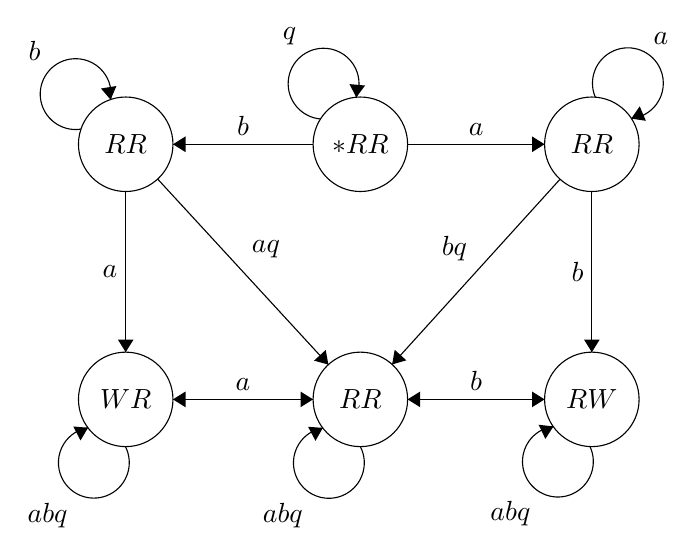
\begin{tikzpicture}[scale=0.2]
    \tikzstyle{every node}+=[inner sep=0pt]
    \draw [black] (8.5,-48.9) circle (3);
    \draw (8.5,-48.9) node {$WR$};
    \draw [black] (23.4,-48.9) circle (3);
    \draw (23.4,-48.9) node {$RR$};
    \draw [black] (38.1,-48.9) circle (3);
    \draw (38.1,-48.9) node {$RW$};
    \draw [black] (8.5,-32.7) circle (3);
    \draw (8.5,-32.7) node {$RR$};
    \draw [black] (23.4,-32.7) circle (3);
    \draw (23.4,-32.7) node {$*RR$};
    \draw [black] (38.1,-32.7) circle (3);
    \draw (38.1,-32.7) node {$RR$};
    \draw [black] (8.476,-51.888) arc (27.27123:-260.72877:2.25);
    \draw (3.54,-55.44) node [below] {$abq$};
    \fill [black] (6.11,-50.7) -- (5.17,-50.62) -- (5.63,-51.51);
    \draw [black] (23.394,-51.888) arc (27.62144:-260.37856:2.25);
    \draw (18.48,-55.46) node [below] {$abq$};
    \fill [black] (21.02,-50.71) -- (20.08,-50.64) -- (20.55,-51.53);
    \draw [black] (37.977,-51.886) arc (25.36938:-262.63062:2.25);
    \draw (32.93,-55.33) node [below] {$abq$};
    \fill [black] (35.66,-50.62) -- (34.72,-50.51) -- (35.15,-51.41);
    \draw [black] (26.4,-48.9) -- (35.1,-48.9);
    \fill [black] (35.1,-48.9) -- (34.3,-48.4) -- (34.3,-49.4);
    \draw (30.75,-48.4) node [above] {$b$};
    \draw [black] (20.4,-48.9) -- (11.5,-48.9);
    \fill [black] (11.5,-48.9) -- (12.3,-49.4) -- (12.3,-48.4);
    \draw (15.95,-48.4) node [above] {$a$};
    \draw [black] (11.5,-48.9) -- (20.4,-48.9);
    \fill [black] (20.4,-48.9) -- (19.6,-48.4) -- (19.6,-49.4);
    \draw [black] (35.1,-48.9) -- (26.4,-48.9);
    \fill [black] (26.4,-48.9) -- (27.2,-49.4) -- (27.2,-48.4);
    \draw [black] (8.5,-35.7) -- (8.5,-45.9);
    \fill [black] (8.5,-45.9) -- (9,-45.1) -- (8,-45.1);
    \draw (8,-40.8) node [left] {$a$};
    \draw [black] (5.671,-31.737) arc (278.9367:-9.0633:2.25);
    \draw (2.71,-27.44) node [above] {$b$};
    \fill [black] (7.54,-29.87) -- (7.91,-29) -- (6.93,-29.16);
    \draw [black] (20.4,-32.7) -- (11.5,-32.7);
    \fill [black] (11.5,-32.7) -- (12.3,-33.2) -- (12.3,-32.2);
    \draw (15.95,-32.2) node [above] {$b$};
    \draw [black] (20.879,-31.095) arc (265.25323:-22.74677:2.25);
    \draw (18.9,-26.43) node [above] {$q$};
    \fill [black] (23.14,-29.72) -- (23.7,-28.97) -- (22.71,-28.88);
    \draw [black] (26.4,-32.7) -- (35.1,-32.7);
    \fill [black] (35.1,-32.7) -- (34.3,-32.2) -- (34.3,-33.2);
    \draw (30.75,-32.2) node [above] {$a$};
    \draw [black] (38.325,-29.72) arc (203.42077:-84.57923:2.25);
    \draw (42.48,-26.39) node [above] {$a$};
    \fill [black] (40.6,-31.07) -- (41.53,-31.21) -- (41.14,-30.29);
    \draw [black] (38.1,-35.7) -- (38.1,-45.9);
    \fill [black] (38.1,-45.9) -- (38.6,-45.1) -- (37.6,-45.1);
    \draw (37.6,-40.8) node [left] {$b$};
    \draw [black] (10.53,-34.91) -- (21.37,-46.69);
    \fill [black] (21.37,-46.69) -- (21.2,-45.76) -- (20.46,-46.44);
    \draw (16.48,-39.34) node [right] {$aq$};
    \draw [black] (36.08,-34.92) -- (25.42,-46.68);
    \fill [black] (25.42,-46.68) -- (26.32,-46.42) -- (25.58,-45.75);
    \draw (30.21,-39.34) node [left] {$bq$};
    \end{tikzpicture}
    \end{center}

    This is an epistemic model: NO \\
    This is a doxasic model: YES \\

\end{enumerate}


%%%%%%%%%%%%%%%%
%% Exercise 2 %%
%%%%%%%%%%%%%%%%
\section*{Exercise 2}

\begin{enumerate}

    \item Representation of the bits world as an epistemic model \textbf{M}: \\

    \begin{center}
    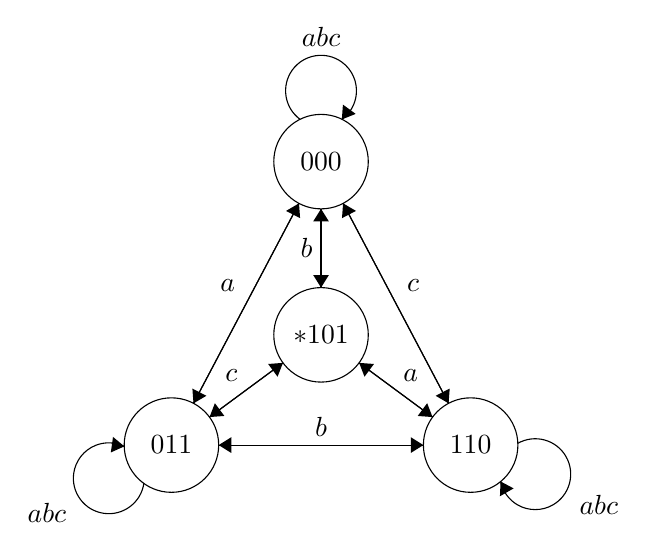
\begin{tikzpicture}[scale=0.2]
    \tikzstyle{every node}+=[inner sep=0pt]
    \draw [black] (39.9,-16.8) circle (3);
    \draw (39.9,-16.8) node {$000$};
    \draw [black] (39.9,-27.8) circle (3);
    \draw (39.9,-27.8) node {$*101$};
    \draw [black] (49.4,-34.8) circle (3);
    \draw (49.4,-34.8) node {$110$};
    \draw [black] (30.4,-34.8) circle (3);
    \draw (30.4,-34.8) node {$011$};
    \draw [black] (28.65,-37.223) arc (-8.10273:-296.10273:2.25);
    \draw (23.75,-39.12) node [left] {$abc$};
    \fill [black] (27.41,-34.88) -- (26.69,-34.28) -- (26.55,-35.27);
    \draw [black] (52.386,-34.694) arc (119.76798:-168.23202:2.25);
    \draw (56.28,-38.57) node [right] {$abc$};
    \fill [black] (51.3,-37.11) -- (51.26,-38.05) -- (52.13,-37.55);
    \draw [black] (38.577,-14.12) arc (234:-54:2.25);
    \draw (39.9,-9.55) node [above] {$abc$};
    \fill [black] (41.22,-14.12) -- (42.1,-13.77) -- (41.29,-13.18);
    \draw [black] (31.8,-32.15) -- (38.5,-19.45);
    \fill [black] (38.5,-19.45) -- (37.68,-19.93) -- (38.57,-20.39);
    \draw (34.47,-24.64) node [left] {$a$};
    \draw [black] (38.5,-19.45) -- (31.8,-32.15);
    \fill [black] (31.8,-32.15) -- (32.62,-31.67) -- (31.73,-31.21);
    \draw [black] (33.4,-34.8) -- (46.4,-34.8);
    \fill [black] (46.4,-34.8) -- (45.6,-34.3) -- (45.6,-35.3);
    \draw [black] (46.4,-34.8) -- (33.4,-34.8);
    \fill [black] (33.4,-34.8) -- (34.2,-35.3) -- (34.2,-34.3);
    \draw (39.9,-34.3) node [above] {$b$};
    \draw [black] (41.3,-19.45) -- (48,-32.15);
    \fill [black] (48,-32.15) -- (48.07,-31.21) -- (47.18,-31.67);
    \draw (45.33,-24.64) node [right] {$c$};
    \draw [black] (48,-32.15) -- (41.3,-19.45);
    \fill [black] (41.3,-19.45) -- (41.23,-20.39) -- (42.12,-19.93);
    \draw [black] (46.98,-33.02) -- (42.32,-29.58);
    \fill [black] (42.32,-29.58) -- (42.66,-30.46) -- (43.26,-29.65);
    \draw (45.6,-30.8) node [above] {$a$};
    \draw [black] (42.32,-29.58) -- (46.98,-33.02);
    \fill [black] (46.98,-33.02) -- (46.64,-32.14) -- (46.04,-32.95);
    \draw [black] (39.9,-24.8) -- (39.9,-19.8);
    \fill [black] (39.9,-19.8) -- (39.4,-20.6) -- (40.4,-20.6);
    \draw [black] (39.9,-19.8) -- (39.9,-24.8);
    \fill [black] (39.9,-24.8) -- (40.4,-24) -- (39.4,-24);
    \draw (39.4,-22.3) node [left] {$b$};
    \draw [black] (32.82,-33.02) -- (37.48,-29.58);
    \fill [black] (37.48,-29.58) -- (36.54,-29.65) -- (37.14,-30.46);
    \draw [black] (37.48,-29.58) -- (32.82,-33.02);
    \fill [black] (32.82,-33.02) -- (33.76,-32.95) -- (33.16,-32.14);
    \draw (34.2,-30.8) node [above] {$c$};
    \end{tikzpicture}
    \end{center}

    \item Representation of event model $\Sigma$:

    \begin{center}
    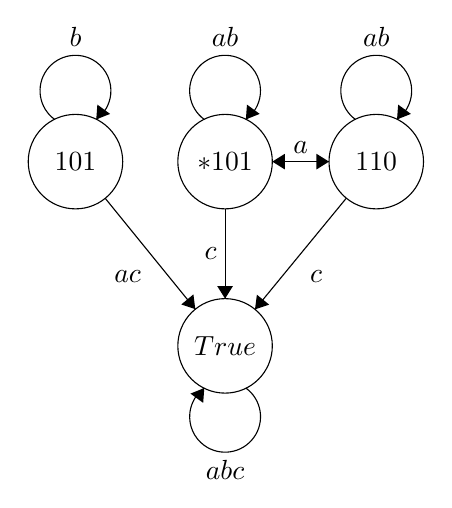
\begin{tikzpicture}[scale=0.2]
    \tikzstyle{every node}+=[inner sep=0pt]
    \draw [black] (9.4,-37.3) circle (3);
    \draw (9.4,-37.3) node {$101$};
    \draw [black] (18.9,-37.3) circle (3);
    \draw (18.9,-37.3) node {$*101$};
    \draw [black] (28.5,-37.3) circle (3);
    \draw (28.5,-37.3) node {$110$};
    \draw [black] (18.9,-49) circle (3);
    \draw (18.9,-49) node {$True$};
    \draw [black] (8.077,-34.62) arc (234:-54:2.25);
    \draw (9.4,-30.05) node [above] {$b$};
    \fill [black] (10.72,-34.62) -- (11.6,-34.27) -- (10.79,-33.68);
    \draw [black] (17.577,-34.62) arc (234:-54:2.25);
    \draw (18.9,-30.05) node [above] {$ab$};
    \fill [black] (20.22,-34.62) -- (21.1,-34.27) -- (20.29,-33.68);
    \draw [black] (27.177,-34.62) arc (234:-54:2.25);
    \draw (28.5,-30.05) node [above] {$ab$};
    \fill [black] (29.82,-34.62) -- (30.7,-34.27) -- (29.89,-33.68);
    \draw [black] (25.5,-37.3) -- (21.9,-37.3);
    \fill [black] (21.9,-37.3) -- (22.7,-37.8) -- (22.7,-36.8);
    \draw (23.7,-36.8) node [above] {$a$};
    \draw [black] (11.29,-39.63) -- (17.01,-46.67);
    \fill [black] (17.01,-46.67) -- (16.89,-45.73) -- (16.12,-46.37);
    \draw (13.59,-44.58) node [left] {$ac$};
    \draw [black] (20.223,-51.68) arc (54:-234:2.25);
    \draw (18.9,-56.25) node [below] {$abc$};
    \fill [black] (17.58,-51.68) -- (16.7,-52.03) -- (17.51,-52.62);
    \draw [black] (26.6,-39.62) -- (20.8,-46.68);
    \fill [black] (20.8,-46.68) -- (21.7,-46.38) -- (20.92,-45.75);
    \draw (24.26,-44.58) node [right] {$c$};
    \draw [black] (18.9,-40.3) -- (18.9,-46);
    \fill [black] (18.9,-46) -- (19.4,-45.2) -- (18.4,-45.2);
    \draw (18.4,-43.15) node [left] {$c$};
    \draw [black] (21.9,-37.3) -- (25.5,-37.3);
    \fill [black] (25.5,-37.3) -- (24.7,-36.8) -- (24.7,-37.8);
    \end{tikzpicture}
    \end{center}

    \pagebreak
    \item Representation of model \textbf{M'}:

    \begin{center}
    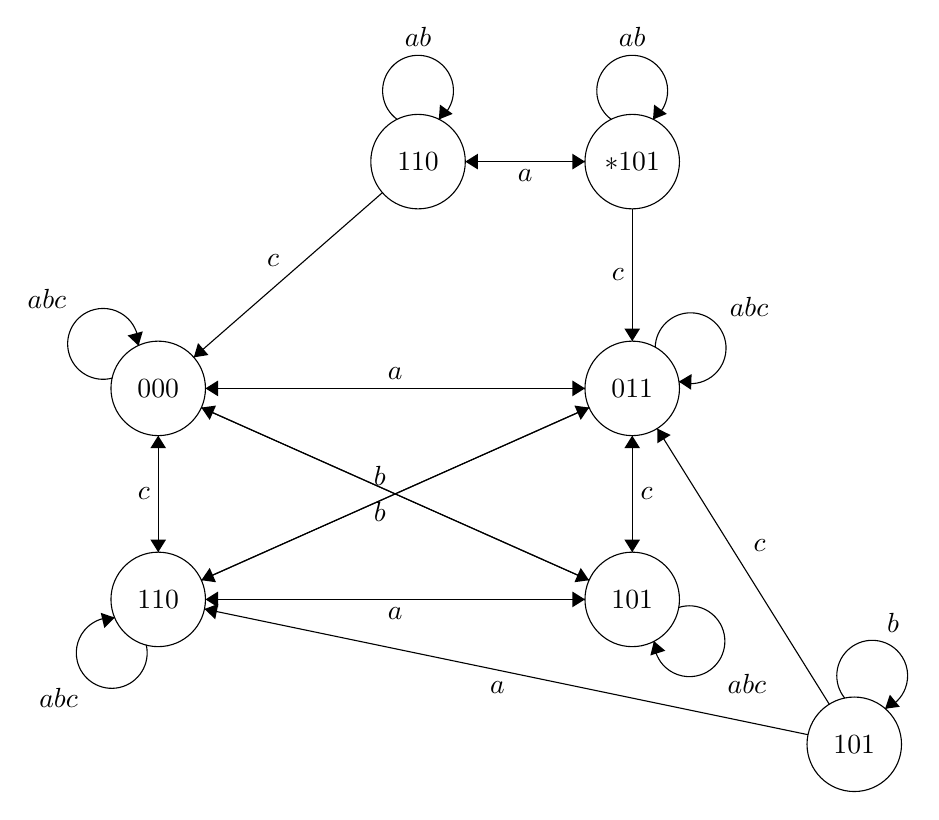
\begin{tikzpicture}[scale=0.2]
    \tikzstyle{every node}+=[inner sep=0pt]
    \draw [black] (55.7,-11.8) circle (3);
    \draw (55.7,-11.8) node {$*101$};
    \draw [black] (42.1,-11.8) circle (3);
    \draw (42.1,-11.8) node {$110$};
    \draw [black] (69.8,-48.8) circle (3);
    \draw (69.8,-48.8) node {$101$};
    \draw [black] (25.6,-26.2) circle (3);
    \draw (25.6,-26.2) node {$000$};
    \draw [black] (55.7,-39.6) circle (3);
    \draw (55.7,-39.6) node {$101$};
    \draw [black] (25.6,-39.6) circle (3);
    \draw (25.6,-39.6) node {$110$};
    \draw [black] (55.7,-26.2) circle (3);
    \draw (55.7,-26.2) node {$011$};
    \draw [black] (54.377,-9.12) arc (234:-54:2.25);
    \draw (55.7,-4.55) node [above] {$ab$};
    \fill [black] (57.02,-9.12) -- (57.9,-8.77) -- (57.09,-8.18);
    \draw [black] (69.199,-45.873) arc (219.3284:-68.6716:2.25);
    \draw (72.26,-41.71) node [above] {$b$};
    \fill [black] (71.76,-46.54) -- (72.69,-46.42) -- (72.06,-45.65);
    \draw [black] (40.777,-9.12) arc (234:-54:2.25);
    \draw (42.1,-4.55) node [above] {$ab$};
    \fill [black] (43.42,-9.12) -- (44.3,-8.77) -- (43.49,-8.18);
    \draw [black] (45.1,-11.8) -- (52.7,-11.8);
    \fill [black] (52.7,-11.8) -- (51.9,-11.3) -- (51.9,-12.3);
    \draw (48.9,-12.3) node [below] {$a$};
    \draw [black] (52.7,-11.8) -- (45.1,-11.8);
    \fill [black] (45.1,-11.8) -- (45.9,-12.3) -- (45.9,-11.3);
    \draw [black] (28.34,-27.42) -- (52.96,-38.38);
    \fill [black] (52.96,-38.38) -- (52.43,-37.6) -- (52.03,-38.51);
    \draw (39.67,-33.41) node [below] {$b$};
    \draw [black] (52.96,-38.38) -- (28.34,-27.42);
    \fill [black] (28.34,-27.42) -- (28.87,-28.2) -- (29.27,-27.29);
    \draw [black] (25.6,-36.6) -- (25.6,-29.2);
    \fill [black] (25.6,-29.2) -- (25.1,-30) -- (26.1,-30);
    \draw [black] (25.6,-29.2) -- (25.6,-36.6);
    \fill [black] (25.6,-36.6) -- (26.1,-35.8) -- (25.1,-35.8);
    \draw (25.1,-32.9) node [left] {$c$};
    \draw [black] (28.6,-26.2) -- (52.7,-26.2);
    \fill [black] (52.7,-26.2) -- (51.9,-25.7) -- (51.9,-26.7);
    \draw (40.65,-25.7) node [above] {$a$};
    \draw [black] (52.7,-26.2) -- (28.6,-26.2);
    \fill [black] (28.6,-26.2) -- (29.4,-26.7) -- (29.4,-25.7);
    \draw [black] (28.6,-39.6) -- (52.7,-39.6);
    \fill [black] (52.7,-39.6) -- (51.9,-39.1) -- (51.9,-40.1);
    \draw (40.65,-40.1) node [below] {$a$};
    \draw [black] (52.7,-39.6) -- (28.6,-39.6);
    \fill [black] (28.6,-39.6) -- (29.4,-40.1) -- (29.4,-39.1);
    \draw [black] (55.7,-36.6) -- (55.7,-29.2);
    \fill [black] (55.7,-29.2) -- (55.2,-30) -- (56.2,-30);
    \draw (56.2,-32.9) node [right] {$c$};
    \draw [black] (55.7,-29.2) -- (55.7,-36.6);
    \fill [black] (55.7,-36.6) -- (56.2,-35.8) -- (55.2,-35.8);
    \draw [black] (28.34,-38.38) -- (52.96,-27.42);
    \fill [black] (52.96,-27.42) -- (52.03,-27.29) -- (52.43,-28.2);
    \draw [black] (52.96,-27.42) -- (28.34,-38.38);
    \fill [black] (28.34,-38.38) -- (29.27,-38.51) -- (28.87,-37.6);
    \draw (39.67,-32.39) node [above] {$b$};
    \draw [black] (39.84,-13.77) -- (27.86,-24.23);
    \fill [black] (27.86,-24.23) -- (28.79,-24.08) -- (28.13,-23.32);
    \draw (32.89,-18.51) node [above] {$c$};
    \draw [black] (55.7,-14.8) -- (55.7,-23.2);
    \fill [black] (55.7,-23.2) -- (56.2,-22.4) -- (55.2,-22.4);
    \draw (55.2,-19) node [left] {$c$};
    \draw [black] (66.86,-48.19) -- (28.54,-40.21);
    \fill [black] (28.54,-40.21) -- (29.22,-40.86) -- (29.42,-39.88);
    \draw (47.14,-44.78) node [below] {$a$};
    \draw [black] (68.21,-46.25) -- (57.29,-28.75);
    \fill [black] (57.29,-28.75) -- (57.29,-29.69) -- (58.14,-29.16);
    \draw (63.38,-36.21) node [right] {$c$};
    \draw [black] (22.684,-25.545) arc (285.06342:-2.93658:2.25);
    \draw (19.79,-20.53) node [left] {$abc$};
    \fill [black] (24.35,-23.49) -- (24.62,-22.58) -- (23.66,-22.84);
    \draw [black] (24.841,-42.49) arc (13.02199:-274.97801:2.25);
    \draw (19.27,-45.19) node [below] {$abc$};
    \fill [black] (22.84,-40.76) -- (21.95,-40.45) -- (22.18,-41.42);
    \draw [black] (58.644,-40.114) arc (107.82974:-180.17026:2.25);
    \draw (61.73,-44.97) node [right] {$abc$};
    \fill [black] (57.08,-42.25) -- (56.85,-43.16) -- (57.8,-42.86);
    \draw [black] (57.159,-23.592) arc (178.51244:-109.48756:2.25);
    \draw (61.86,-21.02) node [right] {$abc$};
    \fill [black] (58.66,-25.77) -- (59.44,-26.29) -- (59.47,-25.29);
    \end{tikzpicture}
    \end{center}




    \item Representation of event model \textbf{$\Sigma$'}:

    \item The update product of the two models \textbf{M''} = \textbf{M}
    $\bigotimes$ \textbf{$\Sigma$'} : \\

\end{enumerate}


%%%%%%%%%%%%%%%%
%% Exercise 3 %%
%%%%%%%%%%%%%%%%
\section*{Exercise 3}

\begin{enumerate}

    \item
    \item
    \item
    \item
    \item
    \item
    \item
    \item
    \item

\end{enumerate}


\end{document}


